\documentclass[11pt,a4paper]{article}
\usepackage[margin=2.2cm]{geometry}
\usepackage[T1]{fontenc}
\usepackage{lmodern}
\usepackage{amsmath,amssymb}
\usepackage{booktabs,tabularx,multirow}
\usepackage{graphicx}
\usepackage{xcolor}
\usepackage[font=small,labelfont=bf]{caption}
\usepackage{subcaption}
\usepackage[ruled,vlined,linesnumbered]{algorithm2e}
\usepackage[numbers,sort&compress]{natbib}
\usepackage[colorlinks=true,linkcolor=teal,citecolor=teal,urlcolor=teal]{hyperref}
\usepackage{enumitem}
\setlist{nosep,leftmargin=*}
\newcommand{\dev}{\mathrm{dev}}
% generated from the notebooks' outputs
\newcommand{\nInstances}{42}
\newcommand{\aOneCHthree}{13.05}
\newcommand{\aOneCHthreeRE}{6.49}
\newcommand{\aOneCHtwo}{19.45}
\newcommand{\aOneCHone}{2,297}
\newcommand{\aTwoCHthreeBI}{2.51}
\newcommand{\aTwoCHthreeFI}{2.83}
\newcommand{\devCHthreeRE}{6.03}
\newcommand{\cpuCHthreeRE}{1.9}
\newcommand{\devBIthreeRE}{2.67}
\newcommand{\cpuBIthreeRE}{22}
\newcommand{\devFIthreeRE}{2.91}
\newcommand{\cpuFIthreeRE}{12}
\newcommand{\devBIthree}{2.48}
\newcommand{\cpuBIthree}{28}
\newcommand{\devSA}{1.34}
\newcommand{\cpuSA}{224}
\newcommand{\devTS}{1.04}
\newcommand{\cpuTS}{230}
\newcommand{\devGAbase}{0.83}
\newcommand{\cpuGAbase}{351}
\newcommand{\ablBase}{1.01}
\newcommand{\ablNoCross}{1.37}
\newcommand{\ablNoMutNoDup}{1.59}
\newcommand{\ablNoRE}{4.00}
\newcommand{\rawInfeasibleInit}{97}
\newcommand{\rawInfeasibleRun}{69}
\newcommand{\tuneBaseShort}{1.07}
\newcommand{\tuneBaseLong}{0.72}
\newcommand{\devGAshort}{1.08}
\newcommand{\cpuGAshort}{231}
\newcommand{\heldGAshort}{1.02}
\newcommand{\hitGAshort}{19}
\newcommand{\devGAlong}{0.76}
\newcommand{\cpuGAlong}{691}
\newcommand{\heldGAlong}{0.79}
\newcommand{\hitGAlong}{29}
\newcommand{\heldTS}{0.96}
\newcommand{\hitTS}{25}
\newcommand{\heldSA}{1.26}
\newcommand{\hitSA}{19}
\newcommand{\heldGAbase}{0.85}
\newcommand{\hitGAbase}{26}
\newcommand{\friedmanChi}{24.7}
\newcommand{\friedmanP}{1.8\cdot10^{-5}}
\newcommand{\pwTSHolm}{0.77}
\newcommand{\pwTSAbetter}{17}
\newcommand{\pwTSBbetter}{21}
\newcommand{\pwSAHolm}{0.063}
\newcommand{\pwSAAbetter}{25}
\newcommand{\pwSABbetter}{14}
\newcommand{\pwBaseHolm}{8.1\cdot10^{-5}}
\newcommand{\pwBaseAbetter}{0}
\newcommand{\pwBaseBbetter}{23}
\newcommand{\pwLongHolm}{2.2\cdot10^{-5}}
\newcommand{\pwLongAbetter}{27}
\newcommand{\pwLongBbetter}{0}
\newcommand{\mcScpTS}{1.11}
\newcommand{\mcScpGA}{1.02}
\newcommand{\mipScptime}{2.8}
\newcommand{\mipScpopt}{14}
\newcommand{\mipScplpgap}{3.06}
\newcommand{\mcScpraw}{69}
\newcommand{\mcTwoTS}{1.72}
\newcommand{\mcTwoGA}{1.51}
\newcommand{\mipTwotime}{4.2}
\newcommand{\mipTwoopt}{14}
\newcommand{\mipTwolpgap}{1.87}
\newcommand{\mcTworaw}{76}
\newcommand{\mcThreeTS}{2.30}
\newcommand{\mcThreeGA}{2.49}
\newcommand{\mipThreetime}{17.3}
\newcommand{\mipThreeopt}{12}
\newcommand{\mipThreelpgap}{1.86}
\newcommand{\mcThreeraw}{69}
\newcommand{\mcVarTS}{1.54}
\newcommand{\mcVarGA}{1.34}
\newcommand{\mipVartime}{2.1}
\newcommand{\mipVaropt}{14}
\newcommand{\mipVarlpgap}{1.27}
\newcommand{\mcVarraw}{76}


\title{From greedy construction to genetic algorithms:\\ heuristics and metaheuristics for the Set Covering Problem}
\author{Group 11: Artur Santoalha, Kirill Savin\\[2pt] \small Heuristic Optimization -- Master in Data Science and Engineering}
\date{November 2026}

\begin{document}
\maketitle

\begin{abstract}
We study the weighted Set Covering Problem (SCP) on the 42 classical OR-Library instances of sets 4, 5, 6 and A--D with a sequence of increasingly powerful methods that share one incrementally updated solution representation:
dynamic constructive heuristics with redundancy elimination (RE), first- and best-improvement local search on a drop-and-repair neighbourhood, simulated annealing (SA), tabu search (TS) and a genetic algorithm (GA) whose crossover keeps the columns two parents share and repairs the offspring.
All methods are evaluated with fixed seeds in paired designs, at controlled budgets and with non-parametric tests.
On average the greedy heuristic with RE is \devCHthreeRE\,\% above the best known values, local search 2.5--2.9\,\%, SA \devSA\,\% and TS \devTS\,\%.
Given exactly the CPU time of tabu search, the GA reaches \devGAshort\,\% and is statistically indistinguishable from TS; with three times that time it reaches \devGAlong\,\% and the best known value on \hitGAlong{} of the 42 instances.
A two-stage tuning study at equal CPU time (4060 runs) shows that only the population size matters significantly -- its best value depends on the budget because the initial population consumes most of a short one -- while all other parameters form a flat plateau, so the baseline configuration is kept.
As an extension we adapt TS and the GA to the multicover problem, where every element must be covered several times; both remain within 1--2.5\,\% of the optima computed by a MIP solver.
\end{abstract}

% =====================================================================================================
\section{Introduction}
Given a ground set of $m$ elements and $n$ subsets with costs, the Set Covering Problem asks for a cheapest collection of subsets that covers every element.
It models crew scheduling, facility location and many other selection problems, and it is NP-hard \cite{garey1979}.
Exact methods solve moderate instances, but heuristics remain the tool of choice for large ones and are the building blocks of most metaheuristics \cite{caprara2000}.

This report summarises four consecutive studies on the same benchmark and with the same code base:
(i) constructive heuristics and redundancy elimination;
(ii) iterative improvement with first and best improvement;
(iii) the neighbourhood-based metaheuristics simulated annealing and tabu search, including a factorial study of their parameters and building blocks;
(iv) a population-based metaheuristic -- a genetic algorithm -- with its design, a working version, parameter tuning and a fair quality-versus-effort comparison with all earlier methods.
Finally, (v) we adapt the two best metaheuristics to the \emph{multicover} extension of the SCP.

Our main contributions are a common, incrementally updated solution state that all methods share and that is verified from scratch after every run; a fast redundancy elimination; a repair-based crossover that keeps the columns two parents have in common;
an experimental methodology with paired seeds, equal-CPU-time budgets and held-out confirmation, which protected us from several apparently promising but spurious improvements; and the observation that a modern MIP solver solves these classical instances to optimality, which we use as a reference for the extension.

Section~\ref{sec:problem} defines the problem, the instances and the methodology; Section~\ref{sec:blocks} the common building blocks.
Sections~\ref{sec:construct}--\ref{sec:ga} present the four studies, Section~\ref{sec:comparison} compares all methods and Section~\ref{sec:multicover} the multicover extension. Section~\ref{sec:discussion} discusses the results and Section~\ref{sec:conclusion} concludes.

% =====================================================================================================
\section{Problem, instances and methodology}\label{sec:problem}
\paragraph{Problem.} Let $a_{ij}=1$ if set $j$ contains element $i$, $w_j>0$ the cost of set $j$ and $x_j\in\{0,1\}$ the decision to select it:
\begin{equation}
\min \sum_{j=1}^{n} w_j x_j \quad \text{s.t.}\quad \sum_{j=1}^{n} a_{ij}x_j \ge 1 \quad (i=1,\dots,m), \qquad x_j\in\{0,1\}. \label{eq:scp}
\end{equation}
A cover is \emph{minimal} (or non-redundant) if no selected set can be removed without uncovering an element.

\paragraph{Instances.} We use the 42 OR-Library instances \cite{beasley1990,beasley1987} of Table~\ref{tab:instances}; costs are integers in $[1,100]$.
Quality is measured by the percentage deviation from the best known value $f^*$, $\dev = 100\,(f-f^*)/f^*$, averaged first over seeds and then over instances.
The best known values of the course were confirmed independently: the MIP solver HiGHS \cite{huangfu2018} solves the SCP instances we checked to proven optimality in seconds and always returns exactly these values (Section~\ref{sec:multicover}).

\begin{table}[t]
\centering\small
\caption{OR-Library instances used in all studies (costs $w_j\in[1,100]$). Density = share of non-zero $a_{ij}$.}
\label{tab:instances}
\begin{tabular}{lrrrrr}
\toprule
Set & \# inst. & $m$ & $n$ & density [\%] & best known $f^*$ \\
\midrule
4 & 8 & 200 & 1000 & 2.0 & 430--641 \\
5 & 9 & 200 & 2000 & 2.0 & 211--302 \\
6 & 5 & 200 & 1000 & 5.0 & 131--161 \\
A & 5 & 300 & 3000 & 2.0 & 232--253 \\
B & 5 & 300 & 3000 & 5.0 & 69--80 \\
C & 5 & 400 & 4000 & 2.0 & 215--243 \\
D & 5 & 400 & 4000 & 5.0 & 60--72 \\
\bottomrule
\end{tabular}
\end{table}


\paragraph{Experimental principles.} Every run is controlled by one seed; within a comparison all methods use the same seeds, so with the same seed they start from the same initial solution (\emph{paired} design, a variance-reduction technique).
Effort is measured in evaluated neighbours/individuals and in CPU time (process time; final comparisons run sequentially).
Methods are compared on instance means with the Friedman test and pairwise Wilcoxon signed-rank tests with Holm's correction \cite{demsar2006,holm1979}; parameter effects with ANOVA (instance as block, partial $\eta^2$).
Parameters are tuned on 14 instances (two per set); the remaining 28 instances are \emph{held out} for confirmation and are reported separately in the final comparison.

% =====================================================================================================
\section{Common building blocks}\label{sec:blocks}
\paragraph{Incremental state.} A (partial) solution is a dictionary of arrays: the selected sets (\texttt{in\_sol}, the binary vector $x$), the coverage count of every element (\texttt{cnt}), the number of still uncovered elements of every set (\texttt{new\_cov}), the list of uncovered elements and the cost.
Adding or removing a set touches only its elements and the sets that contain them; a log of operations allows any tried move to be undone without copying the state.
After every run a function recomputes everything from scratch and asserts equality with the incremental bookkeeping, feasibility and (where required) minimality.

\paragraph{Greedy rule.} The dynamic greedy rule of Chv\'atal \cite{chvatal1979} adds the set with the lowest cost per still uncovered element, $w_j/\texttt{new\_cov}_j$, re-evaluated after every step. A \emph{restricted candidate list} of size \texttt{rcl} picks at random among the \texttt{rcl} best sets (GRASP-like randomisation). The same function completes any partial solution and is the \emph{repair} of all later methods.

\paragraph{Redundancy elimination (RE).} RE scans the selected sets by decreasing cost and removes every set whose elements are all covered at least twice. One pass suffices: removals only decrease coverage counts, so a set found necessary cannot become redundant later. All redundant candidates are detected at once by the sparse product $A\cdot[\texttt{cnt}<2]$; the result is identical to the plain scan and 2--4 times faster.

\paragraph{Drop-and-repair neighbourhood.} For a minimal cover $S$, $N(S)=\{\mathrm{RE}(\mathrm{repair}(S\setminus\{j\})) : j\in S\}$: drop one selected set, cover the elements it alone covered with the greedy rule (the dropped set forbidden) and remove the sets that became redundant.
Every neighbour is a feasible, minimal cover, $|N(S)|=|S|$, and one move can replace one expensive set by several cheap ones (or vice versa), which a one-for-one swap cannot.

% =====================================================================================================
\section{Constructive heuristics (Assignment 1)}\label{sec:construct}
Three dynamic heuristics repeatedly add a set until every element is covered; a set is only a candidate if it covers a still uncovered element, so no redundant set is added during the construction.
\textbf{CH1} picks a random uncovered element and a random set covering it (a blind baseline); \textbf{CH2} picks a random uncovered element and the covering set with the best ratio $w_j/\texttt{new\_cov}_j$; \textbf{CH3} is Chv\'atal's greedy rule over all sets, with the approximation guarantee $H(d)\le 1+\ln d$ for the largest set size $d$.
Table~\ref{tab:construct} reports the results on the 42 instances.

\begin{table}[t]
\centering\small
\setlength{\tabcolsep}{5pt}
\caption{Constructive heuristics (Assignment 1, 42 instances, seed 1). Deviation from $f^*$ before and after RE; RE gain = cost reduction by RE (in brackets: mean $\pm$ std over 10 seeds); \# helped = instances where RE removed at least one set.}
\label{tab:construct}
\begin{tabular}{llrrrrr}
\toprule
 & selection rule & dev [\%] & dev + RE [\%] & RE gain [\%] & \# helped & sets removed \\
\midrule
CH1 & random el. / set & 2,297.07 & 1,755.70 & 23.06 (23.02$\pm$0.86) & 42 & 16.6 \\
CH2 & random el., best ratio & 19.45 & 14.99 & 3.71 (3.69$\pm$0.44) & 40 & 4.0 \\
CH3 & best ratio, all sets & 13.05 & 6.49 & 5.78 (6.08$\pm$0.31) & 42 & 7.8 \\
\bottomrule
\end{tabular}
\end{table}


Information in the selection rule matters most: the blind CH1 is two orders of magnitude worse than CH2 and CH3. RE improves 124 of the 126 constructed covers; it removes the most from CH1 and, among the informed rules, more from the greedy CH3 (5.8\,\% of the cost, deviation halved from \aOneCHthree\,\% to \aOneCHthreeRE\,\%) than from CH2 (3.7\,\%), because the greedy rule picks large sets early that later choices make redundant. CH3 + RE gives the lowest cost on 41 of the 42 instances and is the starting point of all later methods.

% =====================================================================================================
\section{Iterative improvement (Assignment 2)}\label{sec:ls}
First improvement (FI) scans the drop-and-repair neighbourhood in random order and moves to the first strictly better neighbour; best improvement (BI) evaluates the whole neighbourhood. Both apply RE after every step and stop in a local optimum. Table~\ref{tab:ls} gives the results from four starting solutions (CH1, CH2, CH3 and CH1 + RE).

\begin{table}[t]
\centering\small
\caption{Iterative improvement (Assignment 2, 42 instances). Final deviation: mean $\pm$ std over 5 seeds of the per-seed averages; steps and evaluated neighbours per run (seed 1); time = total local-search time over the 42 instances.}
\label{tab:ls}
\begin{tabular}{llrrrrr}
\toprule
start & pivot & dev start [\%] & dev final [\%] & steps & evaluations & time [s] \\
\midrule
CH1 & FI & 2,297 & 3.84 $\pm$ 0.23 & 56.2 & 294 & 3.0 \\
CH1 & BI & 2,297 & 4.00 $\pm$ 0.61 & 32.8 & 2,147 & 23.8 \\
CH2 & FI & 19.45 & 3.84 $\pm$ 0.40 & 9.6 & 169 & 1.8 \\
CH2 & BI & 19.45 & 3.65 $\pm$ 0.39 & 5.7 & 415 & 4.6 \\
CH3 & FI & 13.05 & 2.83 $\pm$ 0.21 & 5.5 & 134 & 1.4 \\
CH3 & BI & 13.05 & \textbf{2.51} $\pm$ 0.29 & 3.3 & 286 & 3.0 \\
CH1+RE & FI & 1,756 & 4.01 $\pm$ 0.44 & 54.0 & 298 & 3.2 \\
CH1+RE & BI & 1,756 & 3.86 $\pm$ 0.33 & 32.4 & 2,101 & 23.4 \\
\bottomrule
\end{tabular}
\end{table}


The local search closes most of the gap of the constructions (from \aOneCHthree\,\% to \aTwoCHthreeBI\,\% from CH3), but the starting solution still matters: CH3 starts give significantly better local optima than CH2 starts (Wilcoxon $p<0.01$ for FI and BI), and the random CH1 starts need ten times more steps.
The running time is proportional to the number of evaluated neighbours (0.18--0.32\,ms per neighbour, depending on the instance set); FI needs 2--7 times fewer evaluations than BI, whereas BI is better only from good starts and only slightly (CH3: \aTwoCHthreeBI\,\% vs.\ \aTwoCHthreeFI\,\%). Only the two CH3-based methods are on the quality--time Pareto front.
Cleaning a random start with RE does not help consistently (CH1 vs.\ CH1 + RE: FI worse, BI not significantly different), because the first moves remove the redundancy anyway.

% =====================================================================================================
\section{Simulated annealing and tabu search (Assignment 3)}\label{sec:sa_ts}
\paragraph{Design.} Both methods start from CH3 + RE, use the drop-and-repair move with RE after every move and a budget of 3000 evaluated neighbours.
\textbf{SA} \cite{kirkpatrick1983} proposes a random neighbour and accepts a worsening $\Delta$ with probability $e^{-\Delta/T}$; $T_0$ is calibrated so that an average worsening move of the start is accepted with probability $p_0$, and $T$ is reduced geometrically, $T\leftarrow\alpha T$, every $L$ evaluations.
\textbf{TS} \cite{glover1989} evaluates a random sample of $k$ neighbours and moves to the best admissible one even if it is worse; sets removed by a move may not be re-added and added sets may not be dropped for a (randomised) tenure; a tabu move is admissible if it improves the best solution (aspiration); a frequency-based penalty is available as long-term memory.

\paragraph{Experiments.} Full factorial grids of the parameters (SA: $p_0\times\alpha\times L$, 72 configurations; TS: tenure $\times\, k$, 30 configurations), one-factor-at-a-time studies of the building blocks, a confirmation of candidate changes on the held-out instances, a budget study and a final comparison on all 42 instances with 10 seeds (Figure~\ref{fig:sats}).

\begin{figure}[t]
\centering
\includegraphics[width=\textwidth]{figures/sa_ts_heatmaps.pdf}
\caption{Average deviation [\%] on the 14 tuning instances. Left: SA by initial acceptance probability $p_0$ and epoch length $L$ (mean over $\alpha$). Right: TS by tenure and sub-neighbourhood size $k$.}
\label{fig:sats}
\end{figure}

\paragraph{Findings.}
\begin{itemize}
\item \textbf{SA:} the start temperature dominates (partial $\eta^2=0.049$; the cooling ratio alone is not significant, $\eta^2=0.0005$). Hot starts never cool down within the budget; the best configurations ($p_0=0.01$, $\alpha=0.95$, $L=200$) accept 10--15\,\% of the proposed moves and form a statistically flat plateau.
\item \textbf{TS:} tenure ($\eta^2=0.33$), $k$ ($0.22$) and their interaction ($0.18$) all matter; long tenures freeze large parts of the cover. Best: tenure 3, $k=20$; evaluating the whole neighbourhood is worse because it allows 2.6 times fewer iterations.
\item \textbf{RE after every move} is the most important building block: without it SA and TS are 1.5--1.6 percentage points (pp) worse, and still 1.3--1.4 pp worse when the cheaper moves are given the same CPU time.
\item \textbf{Winner's curse:} two changes that looked better on the tuning instances (a tabu attribute and a randomised repair) vanished on the held-out instances (Holm $p\ge 0.35$); only confirmed changes were adopted.
\item \textbf{Budget:} TS keeps improving with more evaluations (0.99\,\% $\to$ 0.56\,\% from 3000 to 30\,000 on the tuning instances), whereas SA saturates unless its cooling schedule is scaled with the budget.
\end{itemize}
In the final comparison TS (\devTS\,\%) is significantly better than SA (\devSA\,\%), and both halve the error of the local search at 10--20 times its CPU time.

% =====================================================================================================
\section{A genetic algorithm (Assignment 4)}\label{sec:ga}
\subsection{Choice of the family and design}
Among the population-based families, a GA has the most natural answers for the SCP: a solution is a set of columns, i.e.\ a binary vector; columns shared by two good covers are meaningful building blocks; and the repair and RE of the previous studies turn any union of columns into a feasible, minimal cover.
A BRKGA would need an indirect decoder, ACO constructs every solution from scratch, and a binary PSO has no natural "move towards the best" for sets.
The design decisions are:
\begin{itemize}
\item \textbf{Representation:} $x\in\{0,1\}^n$; decoded in one step ($\texttt{cnt}=A^\top x$) into the incremental state.
\item \textbf{Feasibility:} crossover and mutation can produce infeasible vectors (\rawInfeasibleInit\,\% of the raw children of the initial population, about \rawInfeasibleRun\,\% over a run); they are always \emph{repaired} with the greedy rule and reduced by RE -- every individual is a feasible, minimal cover, so no penalty is needed.
\item \textbf{Evaluation and selection:} minimise the cost; binary tournament.
\item \textbf{Initial population:} one CH3 + RE individual and $N-1$ randomised-greedy + RE individuals with a random candidate-list size $2,\dots,\texttt{rcl\_init}$; duplicates are rejected.
\item \textbf{New solutions:} with probability $p_c$ a \emph{corrected crossover} keeps every set chosen by both parents and assigns each set chosen by only one parent to one of the two children at random, followed by repair and RE; each child is mutated with probability $p_m$ by the drop-and-repair move.
\item \textbf{Population update and diversity:} generational replacement with elitism; a child identical to a member of the new population is mutated (duplicate control).
\item \textbf{Stopping:} part 1: $\xi=30$ generations without improvement; part 2: a CPU-time budget.
\end{itemize}
Algorithm~\ref{alg:ga} summarises one run.

\begin{algorithm}[t]
\caption{Genetic algorithm for the SCP (one run)}\label{alg:ga}
\DontPrintSemicolon
\KwIn{instance; $N$, elite, $p_c$, $p_m$, tournament size $k$, budget}
$P \leftarrow \{\text{CH3+RE}\}\cup\{N-1 \text{ randomised greedy + RE individuals}\}$ (no duplicates)\;
$x^* \leftarrow \arg\min_{x\in P} w^\top x$\;
\While{budget not exhausted}{
  $P' \leftarrow$ the \emph{elite} best individuals of $P$\;
  \While{$|P'|<N$}{
    $p_1,p_2 \leftarrow$ two binary tournaments on $P$\;
    \eIf{$\mathrm{rand}()<p_c$}{
      $c_1 \leftarrow (p_1\wedge p_2)\vee\big((p_1\oplus p_2)\wedge r\big)$, $c_2 \leftarrow (p_1\wedge p_2)\vee\big((p_1\oplus p_2)\wedge\neg r\big)$ for a random mask $r$\;
      repair $c_1,c_2$ with the greedy rule; apply RE\;
    }{$(c_1,c_2)\leftarrow(p_1,p_2)$}
    \ForEach{child $c$}{
      with probability $p_m$: $c\leftarrow$ drop-and-repair$(c)$\;
      \lIf{$c$ duplicates a member of $P'$}{$c\leftarrow$ drop-and-repair$(c)$}
      $P'\leftarrow P'\cup\{c\}$\;
    }
  }
  $P\leftarrow P'$; update $x^*$\;
}
\Return $x^*$ (feasible and minimal)
\end{algorithm}

\subsection{Working version and components}
The working version was verified end to end: the best solution is recomputed from scratch and, independently, from a fresh parse of the instance file; a seed reproduces a run exactly.
An ablation of the untuned baseline ($N=30$) on six instances shows that RE is essential (about four times worse without it), that crossover contributes clearly (\ablBase\,\% with it, \ablNoCross\,\% without it) and that diversity maintenance is needed: without random mutation the result is unchanged only because the duplicate control still mutates copies (more than a quarter of the children); without both the deviation rises to \ablNoMutNoDup\,\%.
Part 1 also revealed \emph{premature convergence}: the diversity of the population (mean Jaccard distance between individuals) falls from 0.31 to 0.13 within a few generations and the best solution is typically found in the first ten generations.
With the stagnation rule the baseline GA reaches \devGAbase\,\% on all 42 instances, but uses \cpuGAbase\,ms per run, 1.5 times the time of TS, and its evaluations cost 2.7 times those of TS.

\subsection{Parameter tuning and improvement}
\paragraph{Protocol.} Following the assignment, the baseline was fixed before tuning ($N=30$, elite 2, $p_c=0.9$, $p_m=0.2$, binary tournament, initial candidate lists up to 5, greedy repair).
We studied nine factors (Table~\ref{tab:tuning}): the seven parameters and two \emph{improvement components} aimed at premature convergence -- a partial restart (after $r$ generations without improvement the elite is kept and the rest rebuilt with randomised greedy + RE) and a memetic step (a child is improved by the first-improvement local search of Section~\ref{sec:ls} with probability $p_{LS}$).
Evaluations do not cost the same in all configurations (an initial individual or a restart is a full construction, a local-search step only one neighbour), so configurations are compared at \emph{equal CPU time}: one and three times the CPU time that TS needs on the instance (0.16--0.38\,s), with the stagnation rule switched off.
\textbf{Experiment A} changes one factor at a time (3500 runs: 14 tuning instances, seeds 101--105, both budgets). A level is adopted only if it is better than the baseline with Holm $p<0.05$.
\textbf{Experiment B} then adds the \emph{promising} changes (at least 0.1\,pp better and better on more instances than worse, but not significant) one at a time, strongest first, on fresh seeds 106--110 (560 runs); whatever is adopted must finally be confirmed on the 28 held-out instances.
The tuning runs use seven parallel worker processes with process-time limits.

\begin{table}[t]
\centering\footnotesize
\setlength{\tabcolsep}{3pt}
\caption{Experiment A: average deviation [\%] of every level at equal CPU time (14 tuning instances $\times$ 5 seeds). Underlined: baseline level; bold: best level; $^{*}$/$^{\times}$: significantly better/worse than the baseline (Wilcoxon on instance means, Holm-corrected within the factor, $p<0.05$).}
\label{tab:tuning}
\begin{tabular}{lllll}
\toprule
factor & levels & 1$\times$ TS time & 3$\times$ TS time \\
\midrule
population size $N$ & 10 / 20 / 30 / 50 / 100 & 1.52 / \textbf{1.02} / \underline{1.07} / 1.90$^{\times}$ / 2.88$^{\times}$ & 1.36$^{\times}$ / 0.78 / \underline{0.72} / \textbf{0.59} / 0.77 \\
mutation prob.\ $p_m$ & 0.0 / 0.1 / 0.2 / 0.4 & 1.08 / 1.11 / \underline{\textbf{1.07}} / 1.09 & 0.70 / 0.70 / \underline{0.72} / \textbf{0.68} \\
crossover prob.\ $p_c$ & 0.5 / 0.7 / 0.9 / 1.0 & \textbf{1.02} / 1.10 / \underline{1.07} / 1.05 & \textbf{0.67} / 0.71 / \underline{0.72} / 0.68 \\
elite size & 0 / 1 / 2 / 5 & 1.38 / 1.18 / \underline{1.07} / \textbf{0.96} & 0.82 / \textbf{0.71} / \underline{0.72} / 0.72 \\
tournament size $k$ & 2 / 3 / 5 & \underline{1.07} / \textbf{0.94} / 1.02 & \underline{0.72} / \textbf{0.64} / 0.77 \\
initial RCL size & 2 / 3 / 5 / 10 & 1.54 / 1.50 / \underline{1.07} / \textbf{1.00} & 0.89 / 0.87 / \underline{\textbf{0.72}} / 0.72 \\
repair RCL size & 1 / 2 / 3 & \underline{\textbf{1.07}} / 1.15 / 1.26 & \underline{0.72} / \textbf{0.60} / 0.69 \\
restart after (gen.) & off / 10 / 20 & \underline{1.07} / \textbf{1.06} / 1.13 & \underline{0.72} / \textbf{0.52} / 0.56 \\
local-search prob. & 0.0 / 0.05 / 0.2 & \underline{1.07} / 0.96 / \textbf{0.95} & \underline{0.72} / 0.59 / \textbf{0.48} \\
\bottomrule
\end{tabular}
\end{table}


\paragraph{Results of Experiment A.}
\begin{itemize}
\item \textbf{Population size is the only parameter with significant effects, and its best value depends on the budget.} With the TS time, $N=50$ and $N=100$ are significantly worse than $N=30$ (Holm $p=0.038$ and $0.009$): $N=100$ completes on average only half a generation, $N=50$ seven, $N=30$ 21. With three times the time the small population fails instead ($N=10$: 254 generations, but the diversity collapses to 0.11; Holm $p=0.023$), and $N=50$ is the best level (not significant).
\item \textbf{The classical GA parameters form a flat plateau.} Mutation and crossover probability and tournament size change the average deviation by at most 0.13\,pp (Holm $p\ge0.65$). The mutation probability has no effect at all -- the duplicate control already mutates every would-be copy (Section~\ref{sec:ga}).
\item \textbf{The improvement components need time.} With the TS time restarts are hardly triggered (0.6 per run) and the memetic step costs most generations (3 instead of 21). With three times the time every level of both components points to an improvement (memetic step $p_{LS}=0.2$: $-0.23$\,pp, better on 7 instances, worse on 3; restart after 10 generations: $-0.19$\,pp, and the final diversity doubles from 0.15 to 0.29), but none is significant after the correction ($p=0.14$--$0.23$).
\end{itemize}

\begin{figure}[t]
\centering
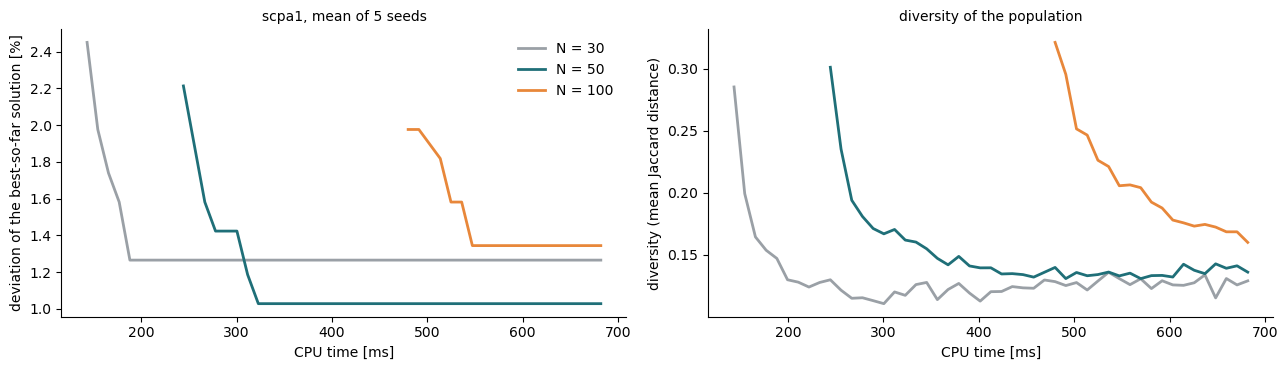
\includegraphics[width=\textwidth]{figures/convergence.png}
\caption{Convergence on \texttt{scpa1} with three times the TS time (mean of 5 seeds): deviation of the best-so-far solution (left) and diversity of the population (right) for $N=30$, $50$ and $100$. The curves start when the initial population is complete. The TS time on this instance is 227\,ms.}
\label{fig:convergence}
\end{figure}

\paragraph{Why the budget decides the population size.} Figure~\ref{fig:convergence} shows the mechanism. The initial population of $N=30$ randomised greedy individuals takes about 140\,ms on \texttt{scpa1} (4.7\,ms per individual), i.e.\ about 60\,\% of the TS time; with $N=50$ or $100$ the initial population alone takes 245 or 480\,ms.
After the initialisation the best solution improves within a few generations and then stagnates while the diversity collapses to about 0.12 -- the premature convergence of part~1. A larger population stays more diverse and ends better when the time allows it ($N=50$: 1.03\,\% vs.\ 1.27\,\% for $N=30$ on this instance), while $N=100$ is still converging when the time runs out.

\begin{table}[t]
\centering\footnotesize
\setlength{\tabcolsep}{4pt}
\caption{Experiment B: the promising changes of Experiment A added one at a time ($C_k = C_{k-1}$ + one change), new seeds 106--110 on the 14 tuning instances, equal CPU time. Better:worse = instances where the configuration has a lower\,/\,higher mean than the reference; Holm-corrected Wilcoxon $p$; generations and final diversity (mean Jaccard distance) per run.}
\label{tab:stageB}
\begin{tabular}{llllrrrrr}
\toprule
budget & config. & change & dev [\%] & diff [pp] & better:worse & Holm $p$ & gen. & div. \\
\midrule
\multirow{3}{*}{1$\times$ TS} & reference & stage-A config.\ (= baseline) & 1.07 &  &  &  & 19 & 0.16 \\
 & C1 & + ls\_prob $=$ 0.2 & 1.03 & $-0.04$ & 4:6 & 0.878 & 3 & 0.26 \\
 & C2 & + elite $=$ 5 & 0.88 & $-0.19$ & 6:4 & 0.569 & 3 & 0.25 \\
\midrule
\multirow{5}{*}{3$\times$ TS} & reference & stage-A config.\ (= baseline) & 0.63 &  &  &  & 97 & 0.15 \\
 & C1 & + ls\_prob $=$ 0.2 & 0.51 & $-0.12$ & 6:4 & 0.641 & 13 & 0.18 \\
 & C2 & + restart\_after $=$ 10 & 0.49 & $-0.14$ & 6:3 & 0.641 & 13 & 0.20 \\
 & C3 & + pop\_size $=$ 50 & 0.50 & $-0.13$ & 6:4 & 0.641 & 7 & 0.24 \\
 & C4 & + rcl\_repair $=$ 2 & 0.45 & $-0.18$ & 7:3 & 0.558 & 6 & 0.25 \\
\bottomrule
\end{tabular}
\end{table}


\paragraph{Experiment B and the decision.} No configuration of the nested sequences is significantly better than the reference (Table~\ref{tab:stageB}); all four long-budget changes together gain 0.18\,pp (better on 7 instances, worse on 3, Holm $p=0.56$).
The effects also \emph{shrank} on the new seeds (memetic step: $-0.23$\,pp in Experiment A, $-0.12$\,pp in B), and the reference itself moved by 0.09\,pp: with 14 instances the seed-to-seed noise is as large as the effects we try to measure.
This is the winner's curse already observed in Assignment~3 -- selecting the best of many levels overestimates its benefit.
\textbf{The baseline values are therefore kept at both budgets}; the GA of the final comparison is the baseline parameter set with a CPU-time stop. This is a result rather than a failure: the baseline, chosen in part~1 from design reasoning, lies on a flat plateau, and the protocol prevented the adoption of changes that do not replicate.
Restarts and the memetic step remain candidates for longer runs, where their effect grows.

% =====================================================================================================
\section{Comparison of all methods}\label{sec:comparison}
All methods were run on the 42 instances with the same 10 seeds (Table~\ref{tab:final}, Figure~\ref{fig:frontier}). Constructions and local search are run to completion, SA and TS use 3000 evaluated neighbours, the part-1 GA stops after 30 generations without improvement, and the GA of part~2 receives exactly the CPU time of the TS run with the same instance and seed (measured CPU time / limit $=1.004$), or three times that time.

\begin{table}[t]
\centering\small
\caption{All methods on the 42 instances with the same 10 seeds (Section~\ref{sec:comparison}). Average deviation over all instances and over the 28 held-out instances, best of 10 runs, mean standard deviation over seeds, number of instances where $f^*$ was reached in at least one run, and CPU time per run.}
\label{tab:final}
\begin{tabular}{lrrrrrr}
\toprule
method & dev [\%] & held-out [\%] & best of 10 [\%] & std & $f^*$ reached & CPU [ms] \\
\midrule
GA, 3$\times$ TS time & 0.76 & 0.79 & 0.22 & 0.43 & 29 & 691.2 \\
GA, 1$\times$ TS time & 1.08 & 1.02 & 0.42 & 0.47 & 19 & 231.3 \\
GA part 1 (stagnation stop) & 0.83 & 0.85 & 0.31 & 0.42 & 26 & 351.2 \\
\midrule
Tabu search & 1.04 & 0.96 & 0.41 & 0.53 & 25 & 229.9 \\
Simulated annealing & 1.34 & 1.26 & 0.69 & 0.55 & 19 & 224.1 \\
\midrule
CH3 + BI & 2.48 & 2.38 & 1.23 & 1.06 & 7 & 28.2 \\
CH3 + RE + BI & 2.67 & 2.54 & 1.23 & 1.15 & 8 & 22.3 \\
CH3 + RE + FI & 2.91 & 2.73 & 1.41 & 1.20 & 7 & 11.8 \\
\midrule
CH3 + RE & 6.03 & 5.83 & 3.91 & 1.53 & 1 & 1.9 \\
CH2 + RE & 14.50 & 14.69 & 7.80 & 4.65 & 0 & 1.0 \\
CH1 + RE & 1,642 & 1,564 & 1,353 & 174.2 & 0 & 1.0 \\
\bottomrule
\end{tabular}
\end{table}


\begin{figure}[t]
\centering
\includegraphics[width=\textwidth]{figures/frontier.pdf}
\caption{Quality versus effort for all methods (42 instances, 10 seeds). Left: every method of Assignments 1--4 with the efficient frontier (dashed); right: the metaheuristics with the standard error over instances. The error bars are wide because the instances differ; the comparisons below are paired.}
\label{fig:frontier}
\end{figure}

\begin{itemize}
\item \textbf{At equal CPU time the GA and tabu search are statistically indistinguishable}: \devGAshort\,\% vs.\ \devTS\,\%, the GA is better on \pwTSAbetter{} instances, TS on \pwTSBbetter{} (Wilcoxon $p=\pwTSHolm$). On the held-out instances the GA reaches \heldGAshort\,\%, TS \heldTS\,\% and SA \heldSA\,\%. Both are better than SA (\devSA\,\%); for the GA the difference is not significant after the Holm correction ($p=\pwSAHolm$), for TS it was ($p<10^{-4}$, Assignment~3). Friedman test over GA (TS time), TS, SA and the part-1 GA: $\chi^2=\friedmanChi$, $p=\friedmanP$.
\item \textbf{The advantage of the part-1 GA over TS came from its larger effort} (\cpuGAbase\,ms vs.\ \cpuTS\,ms per run): with the TS time it disappears. Comparisons at equal \emph{evaluations} flatter the GA even more, because one GA evaluation (a whole new cover: decode, repair, RE) costs 2.7 times a neighbour evaluation of TS or SA.
\item \textbf{More time keeps paying off for the GA}: \devGAshort\,\% $\to$ \devGAbase\,\% $\to$ \devGAlong\,\% at 1, about 1.5 and 3 times the TS time; three times is better than one time on \pwLongAbetter{} instances and never worse (Holm $p=\pwLongHolm$). With three times the TS time the GA reaches the best known value on \hitGAlong{} of 42 instances (TS \hitTS, SA \hitSA) and has the smallest spread over seeds.
\item \textbf{The frontier is a staircase}: every step down in error costs roughly a factor of ten in time -- greedy + RE (6\,\% in 2\,ms), local search (2.5--2.9\,\% in 12--28\,ms), SA/TS/GA (0.8--1.3\,\% in 0.2--0.7\,s). The CH1- and CH2-based local searches are dominated by the CH3-based ones. The GA does not move the frontier down at the TS time; it extends it to the right.
\end{itemize}

% =====================================================================================================
\section{Extension: the multicover problem}\label{sec:multicover}
\paragraph{Problem and assumptions.} In the multicover SCP every element $i$ must be covered by at least $b_i\ge1$ selected sets (e.g.\ backup service), and every set can be selected at most once:
\begin{equation}
\min \sum_{j=1}^{n} w_j x_j \quad \text{s.t.}\quad \sum_{j=1}^{n} a_{ij}x_j \ge b_i \quad (i=1,\dots,m), \qquad x_j\in\{0,1\}.
\end{equation}
An instance is feasible only if $b_i\le\deg(i)$, the number of sets containing $i$. Costs and incidence are those of the 14 tuning instances; four requirement scenarios are generated: \textsf{SCP} ($b_i=1$, reference), \textsf{MC2} ($b_i=2$), \textsf{MC3} ($b_i=3$) and \textsf{MCvar} ($b_i\in\{1,2,3\}$ with probabilities 0.5/0.3/0.2, seeded per instance). Every element lies in at least 9 sets, so the cap $b_i\le\deg(i)$ never binds.
As there are no best known values, every model is solved with HiGHS \cite{huangfu2018} through SciPy \cite{virtanen2020} (60\,s limit), and the heuristics are measured by their gap to its solution.

\paragraph{Adaptation.} We adapt the best method of each family -- TS and the GA. Because both are built on the same building blocks, the adaptation is made once, in the blocks:
an element is \emph{deficient} while $\texttt{cnt}_i<b_i$ (it replaces "uncovered"); the greedy score counts the deficient elements a set would serve; the repair must \emph{exclude already selected sets} (for $b=1$ a selected set is never a candidate because it covers no uncovered element; for $b\ge2$ it can be); a set is redundant if all its elements are covered at least $b_i+1$ times; feasibility is $\texttt{cnt}\ge b$.
Everything above the blocks -- the drop-and-repair move, tabu attributes, aspiration, crossover, mutation, selection and replacement -- is unchanged. With $b\equiv1$ the generalised blocks reproduce TS and the GA exactly, every multicover solution passes the from-scratch check (feasible and minimal), and every heuristic cost lies above the MIP lower bound.

\paragraph{Experiment.} TS (Assignment~3 configuration, 3000 evaluations) and the GA of Section~\ref{sec:ga} run on the 14 instances $\times$ 4 scenarios $\times$ 5 seeds; the GA receives the CPU time that TS used for the same instance, scenario and seed in the same worker process.

\begin{table}[t]
\centering\footnotesize
\setlength{\tabcolsep}{4pt}
\caption{Multicover experiment (14 instances $\times$ 5 seeds). MIP: mean optimal (or best) cost, number of models solved to proven optimality within 60\,s and mean solve time; start: gap of the CH3 + RE start; gap = average gap to the MIP solution; opt.\ = instances where the MIP value was reached in at least one run; GA:TS = instances where the GA / TS mean is lower; $p$ = Wilcoxon test GA vs.\ TS.}
\label{tab:multicover}
\begin{tabular}{lrrrrlrrrrrr}
\toprule
scen. & MIP cost & proven & MIP [s] & start [\%] & method & gap [\%] & opt. & CPU [ms] & sets & GA:TS & $p$ \\
\midrule
\multirow{2}{*}{SCP} & \multirow{2}{*}{227.1} & \multirow{2}{*}{14/14} & \multirow{2}{*}{2.8} & \multirow{2}{*}{6.37} & TS & 1.11 & 8 & 332 & 56.8 &  &  \\
 & & & & & GA & 1.02 & 6 & 333 & 57.4 & 6:5 & 0.695 \\
\midrule
\multirow{2}{*}{MC2} & \multirow{2}{*}{512.1} & \multirow{2}{*}{14/14} & \multirow{2}{*}{4.2} & \multirow{2}{*}{6.17} & TS & 1.72 & 5 & 359 & 95.7 &  &  \\
 & & & & & GA & 1.51 & 4 & 361 & 96.5 & 8:6 & 0.326 \\
\midrule
\multirow{2}{*}{MC3} & \multirow{2}{*}{878.9} & \multirow{2}{*}{12/14} & \multirow{2}{*}{17.3} & \multirow{2}{*}{6.21} & TS & 2.30 & 0 & 378 & 132.5 &  &  \\
 & & & & & GA & 2.49 & 0 & 381 & 134.6 & 6:7 & 0.650 \\
\midrule
\multirow{2}{*}{MCvar} & \multirow{2}{*}{488.0} & \multirow{2}{*}{14/14} & \multirow{2}{*}{2.1} & \multirow{2}{*}{5.49} & TS & 1.54 & 3 & 348 & 89.8 &  &  \\
 & & & & & GA & 1.34 & 3 & 350 & 90.6 & 7:7 & 0.358 \\
\bottomrule
\end{tabular}
\end{table}


\begin{figure}[t]
\centering
\includegraphics[width=0.92\textwidth]{figures/multicover.pdf}
\caption{Multicover: average gap of TS and GA to the MIP solution at equal CPU time (left) and the solve time of HiGHS (right; bars: mean, markers: maximum over the 14 instances).}
\label{fig:multicover}
\end{figure}

\paragraph{Impact on quality and effort.} The CH3 + RE start is about equally far from the optimum in all scenarios (5.5--6.4\,\%), but the metaheuristics close less of this gap as the requirement grows (Table~\ref{tab:multicover}, Figure~\ref{fig:multicover}): TS \mcScpTS{} $\to$ \mcTwoTS{} $\to$ \mcThreeTS\,\% and GA \mcScpGA{} $\to$ \mcTwoGA{} $\to$ \mcThreeGA\,\% for $b=1,2,3$; heterogeneous requirements lie in between.
A cover for $b=3$ holds about 133 sets instead of 57, so one drop-and-repair move changes a much smaller part of the solution, and every evaluation becomes more expensive: in the same time the GA evaluates 1312, 1039 and 756 children for $b=1,2,3$, and TS needs 332 to 378\,ms for its 3000 neighbours.
The exact solver feels the extension more: its mean solve time grows from \mipScptime\,s to \mipThreetime\,s and two of the 14 \textsf{MC3} models are not proven optimal within 60\,s, although the LP gap is \emph{smaller} for multicover (1.9\,\% vs.\ 3.1\,\%).

\paragraph{TS versus GA.} Neither algorithm needed changes of its own logic: the TS move and the GA crossover simply call the generalised repair and RE. Their behaviour differs -- TS makes 3000 cheap local moves, whereas the GA recombines whole covers, and 69--76\,\% of its raw children violate a requirement and need the repair.
At equal CPU time no difference is significant in any scenario (Wilcoxon $p=0.33$--$0.70$): the GA is slightly ahead for $b=1$, $b=2$ and \textsf{MCvar}, TS for $b=3$, where the GA's more expensive children leave it the fewest generations.

% =====================================================================================================
\section{Discussion}\label{sec:discussion}
\paragraph{Fair comparisons.} The most consequential methodological choice was the measure of effort. Counted in evaluations, the GA looked far better than TS (part~1); counted in CPU time it is equal. A GA evaluation builds a whole cover, a TS evaluation changes one set -- comparisons of different families must use time (or another common currency), and the time must include the initialisation: the initial population consumed about 60\,\% of the short budget.

\paragraph{Tuning: flat landscapes and the winner's curse.} In Assignments 3 and 4 the parameter landscapes were largely flat around reasonable values, with a few decisive factors (SA: the start temperature; TS: tenure and sample size; GA: the population size relative to the budget).
Effects of 0.1--0.2\,pp were of the same size as the seed-to-seed variation on 14 instances, and changes that looked best on the tuning runs shrank or vanished on new seeds or held-out instances. Paired designs, multiple-testing corrections and independent confirmation were therefore essential; racing procedures such as F-Race \cite{birattari2010} would spend the runs more efficiently.

\paragraph{Problem-specific components dominate.} Redundancy elimination was the most important building block of every method (constructions, local search, SA, TS, GA), worth from 1.5 to more than 6 percentage points, whereas the GA's own parameters changed the result by at most a few tenths of a point. The greedy repair turns every recombination into a feasible cover; it is also what made the multicover adaptation a matter of a few lines.

\paragraph{The exact-solver perspective.} A modern MIP solver solves the tuning instances to proven optimality in 2.8\,s on average (at most 13\,s) and confirmed all best known values we checked. On these classical sizes the heuristics are about ten times faster but 1\,\% from the optimum; their place is in larger instances, real-time settings and as primal heuristics inside exact methods. Dedicated SCP heuristics from the literature, e.g.\ the GA of Beasley and Chu \cite{beasley1996} or the Lagrangian heuristic of Caprara et al.\ \cite{caprara1999}, reach (near-)best known values on these sets with longer runs and stronger problem knowledge (dual information, column fixing).

\paragraph{Limitations.} Absolute times refer to a Python implementation on one laptop; process time limits are slightly noisy, and the tuning runs shared the machine with six other workers. The tuning set has only 14 instances, the classical OR-Library instances are small, and the multicover requirements are synthetic.

% =====================================================================================================
\section{Conclusions}\label{sec:conclusion}
Starting from a common, verified solution state, we built a sequence of SCP methods in which every stage re-used the previous one: the greedy rule with redundancy elimination (\devCHthreeRE\,\% above the best known values), local search on a drop-and-repair neighbourhood (2.5--2.9\,\%), simulated annealing and tabu search (\devSA\,\% and \devTS\,\%) and a genetic algorithm with a repair-based crossover.
At equal CPU time the GA and TS are statistically equal (\devGAshort\,\% vs.\ \devTS\,\%); with more time the GA keeps improving (\devGAlong\,\% at three times the TS time, best known value on \hitGAlong{} of 42 instances).
The tuning study showed that only the population size, relative to the time budget, matters significantly, and the protocol kept the baseline instead of adopting effects that did not replicate.
The multicover extension required changes only in the shared building blocks; TS and GA stay within 1--2.5\,\% of the MIP optimum, with no significant difference between them.
The main lessons are methodological -- compare at equal CPU time, confirm tuning results on new seeds and instances -- and algorithmic: problem-specific components (greedy repair and RE) matter more than the parameters of the metaheuristic.
Promising directions are a cheaper initial population (e.g.\ mutating one greedy cover instead of $N$ constructions), adaptive population sizes, restarts and memetic steps for longer budgets, and Lagrangian information in the greedy score.

\bibliographystyle{abbrvnat}
\bibliography{references}
\end{document}
